\documentclass[aspectratio=169]{ctexbeamer}
\usepackage{booktabs}
\usepackage{listings}
\usepackage{xcolor}
\usepackage{float}
\usepackage{makecell}
\usetheme{Madrid}

\input{color_style.tex}
\lstdefinelanguage[RISC-V]{Assembler}
{
    alsoletter={.}, % allow dots in keywords
    alsodigit={0x}, % hex numbers are numbers too!
    morekeywords=[1]{ % instructions
            lb, lh, lw, lbu, lhu,
            sb, sh, sw,
            sll, slli, srl, srli, sra, srai,
            add, addi, sub, lui, auipc,
            xor, xori, or, ori, and, andi,
            slt, slti, sltu, sltiu,
            beq, bne, blt, bge, bltu, bgeu, bnez,
            j, jr, jal, jalr, ret,
            scall, break, nop,
            vsetvli,
            vle8.v,
            vse8.v
        },
    morekeywords=[2]{ % sections of our code and other directives
            .align, .ascii, .asciiz, .byte, .data, .double, .extern,
            .float, .globl, .half, .kdata, .ktext, .set, .space, .text, .word
        },
    morekeywords=[3]{ % registers
            zero, ra, sp, gp, tp, s0, fp,
            t0, t1, t2, t3, t4, t5, t6,
            s1, s2, s3, s4, s5, s6, s7, s8, s9, s10, s11,
            a0, a1, a2, a3, a4, a5, a6, a7,
            ft0, ft1, ft2, ft3, ft4, ft5, ft6, ft7,
            fs0, fs1, fs2, fs3, fs4, fs5, fs6, fs7, fs8, fs9, fs10, fs11,
            fa0, fa1, fa2, fa3, fa4, fa5, fa6, fa7
        },
    morecomment=[l]{;},   % mark ; as line comment start
    morecomment=[l]{\#},  % as well as # (even though it is unconventional)
    morestring=[b]",      % mark " as string start/end
    morestring=[b]'       % also mark ' as string start/end
}

% Add "\usepackage{xcolor}"
% define some basic colors
\definecolor{mauve}{rgb}{0.58,0,0.82}

\definecolor{codegreen}{rgb}{0,0.6,0}
\definecolor{codegray}{rgb}{0.5,0.5,0.5}
\definecolor{codepurple}{rgb}{0.58,0,0.82}
\definecolor{backcolour}{rgb}{1,1,1}


\setmonofont{inconsolata}

\lstset{
% listings sonderzeichen (for german weirdness)
literate={ö}{{\"o}}1
{ä}{{\"a}}1
{ü}{{\"u}}1,
basicstyle=\tiny\ttfamily,                    % very small code
breaklines=true,                              % break long lines
commentstyle=\itshape\color{green!50!black},  % comments are green
keywordstyle=[1]\color{blue!80!black},        % instructions are blue
keywordstyle=[2]\color{orange!80!black},      % sections/other directives are orange
keywordstyle=[3]\color{red!50!black},         % registers are red
stringstyle=\color{mauve},                    % strings are from the telekom
identifierstyle=\color{teal},                 % user declared addresses are teal
frame=l,                                      % black line on the left side of code
language=C++,                   % all code is RISC-V
tabsize=4,                                    % indent tabs with 4 spaces
showstringspaces=false                        % do not replace spaces with weird underlines
}

\lstdefinestyle{mystyle}
{
    backgroundcolor=\color{backcolour},
    commentstyle=\color{codegreen},
    keywordstyle=\color{magenta},
    numberstyle=\tiny\color{codegray},
    stringstyle=\color{codepurple},
    basicstyle=\ttfamily\footnotesize,
    breakatwhitespace=false,
    breaklines=true,
    captionpos=b,
    keepspaces=true,
    numbers=none,
    numbersep=5pt,
    showspaces=false,
    showstringspaces=false,
    showtabs=false,
    tabsize=2,
    frame=none
}

\definecolor{orange3}{rgb}{0.425,0.191,0.000}
\definecolor{scarletred3}{rgb}{0.643,0.000,0.000}
\definecolor{green3}{rgb}{0.000,0.405,0.000}
\definecolor{blue3}{rgb}{0.000,0.000,0.704}
\definecolor{aluminium1}{rgb}{0.933,0.933,0.925}
\definecolor{aluminium2}{rgb}{0.827,0.843,0.812}
\definecolor{aluminium3}{rgb}{0.729,0.741,0.714}
\definecolor{aluminium4}{rgb}{0.533,0.541,0.522}
\definecolor{aluminium5}{rgb}{0.333,0.341,0.325}
\definecolor{aluminium6}{rgb}{0.180,0.204,0.212}

\lstdefinelanguage{llvm}{
    % see https://tex.stackexchange.com/questions/137237/listings-text-highlighting-based-on-prefix
    %moredelim=[s][\color{orange3}]{x}{>},
    alsoletter={\%,\#,!},
    basicstyle=\tiny\ttfamily,
    keywordsprefix={\%},
    morekeywords={\%},
    keywordstyle=\color{orange3},
    commentstyle=\color{aluminium4},
    % this allows to color inside <memrefxf32> (i.e., f32).
    otherkeywords={index, f32, i32, f64, i8},
    keywords=[3]{index, f32, memref, i32, f64, i8, affine_map, affine_set, iter_args},
    keywordstyle=[3]\color{scarletred3},
    keywords=[4]{affine},
    keywordstyle=[4]\color{aluminium6},
    showstringspaces=false,
    breaklines=true,
    breakatwhitespace=true,
    morestring=[b]",
    stringstyle=\color{green3},
    moredelim=[s][\color{blue3}]{\#}{<},
    moredelim=[s][\color{scarletred3}]{!}{\ },
    morecomment=[l]{//},
}

\lstset{style=mystyle,language=C++}

\input{section_pages.tex}

\title{Auto Vectorization Methods \& Implementations for Modern Architecture}
\subtitle{现代体系结构自动向量化的方法与实现}
\author{龙英池}
\institute{HIT}

\begin{document}
\maketitle

\begin{frame}
    \frametitle{Table of Contents}

    \tableofcontents

\end{frame}

\section{Moore定律的终结和并行化的需求}

\begin{frame}
    \frametitle{Moore's Law to be over}

    集成电路上可容纳的晶体管数目,约每隔两年便会增加一倍

    \begin{figure}[h]
        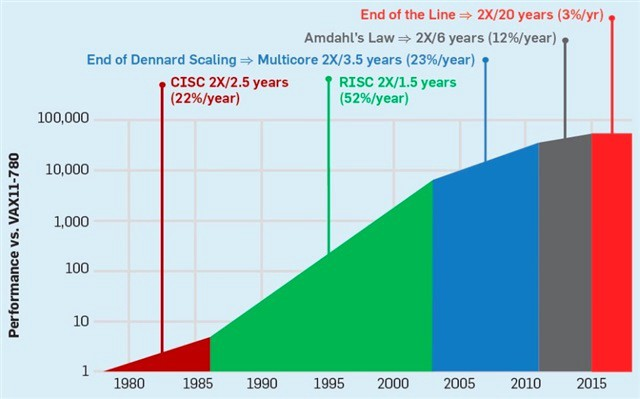
\includegraphics[height=0.5\textheight]{images/moore.jpeg}
        \caption{Moore's Law}
    \end{figure}

\end{frame}

\begin{frame}
    \frametitle{Parallel}

    提高计算机性能的方法,是并行化。

    \begin{figure}[h]
        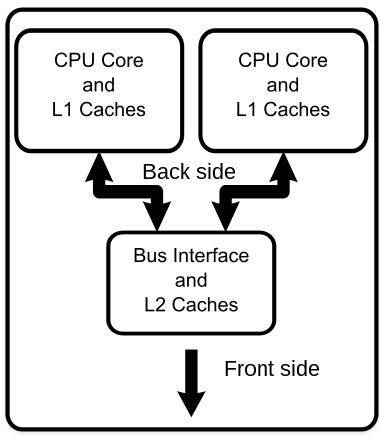
\includegraphics[height=0.5\textheight]{images/dual_core.png}
        \caption{Dual Core Cache Design}
    \end{figure}

\end{frame}

\section{并行的手段}

\subsection{Multi-Core}

\begin{frame}
    \frametitle{Multi-Core}

    为了实现并行化,我们可以给一个计算机加入多个核心。

    \begin{itemize}
        \item 不同的寄存器
        \item 不同的中断处理请求
        \item 操作系统-对称多处理(SMP)调度
    \end{itemize}

    \begin{figure}[h]
        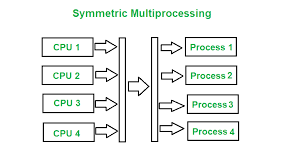
\includegraphics[height=0.45\textheight]{images/smp.png}
        \caption{Symmetric multiprocessing}
    \end{figure}

\end{frame}

\subsection{Single-Core}

\begin{frame}[fragile]
    \frametitle{Single-Core - Out-of-Order Execution}

    乱序执行(Out-of-Order Execution)是现代CPU最基本的一个并行手段。
    \begin{minipage}[t]{0.45\linewidth}
        \begin{lstlisting}[language=C++]
int test(int &a,
         int &b,
         int &c,
         int &d) {
    a += b;
    c += d;
    return 0;
}
        \end{lstlisting}
    \end{minipage}
    \begin{minipage}[t]{0.45\linewidth}
        \begin{lstlisting}[language={[RISC-V]Assembler}]
    lw      a1, 0(a1)
    lw      a4, 0(a0)
    addw    a1, a1, a4
    sw      a1, 0(a0)
    lw      a0, 0(a3)
    lw      a1, 0(a2)
    addw    a0, a0, a1
    sw      a0, 0(a2)
        \end{lstlisting}
    \end{minipage}


\end{frame}

\begin{frame}
    \frametitle{Single-Core - SIMD}

    OoOE在编程上由编译器全局指令调度器(Instruction Scheduler)优化。

    单指令流多数据流(Single instruction, multiple data (SIMD)),提供了一种让我
    们更好地进行向量计算的方式。

    \begin{figure}
        \centering
        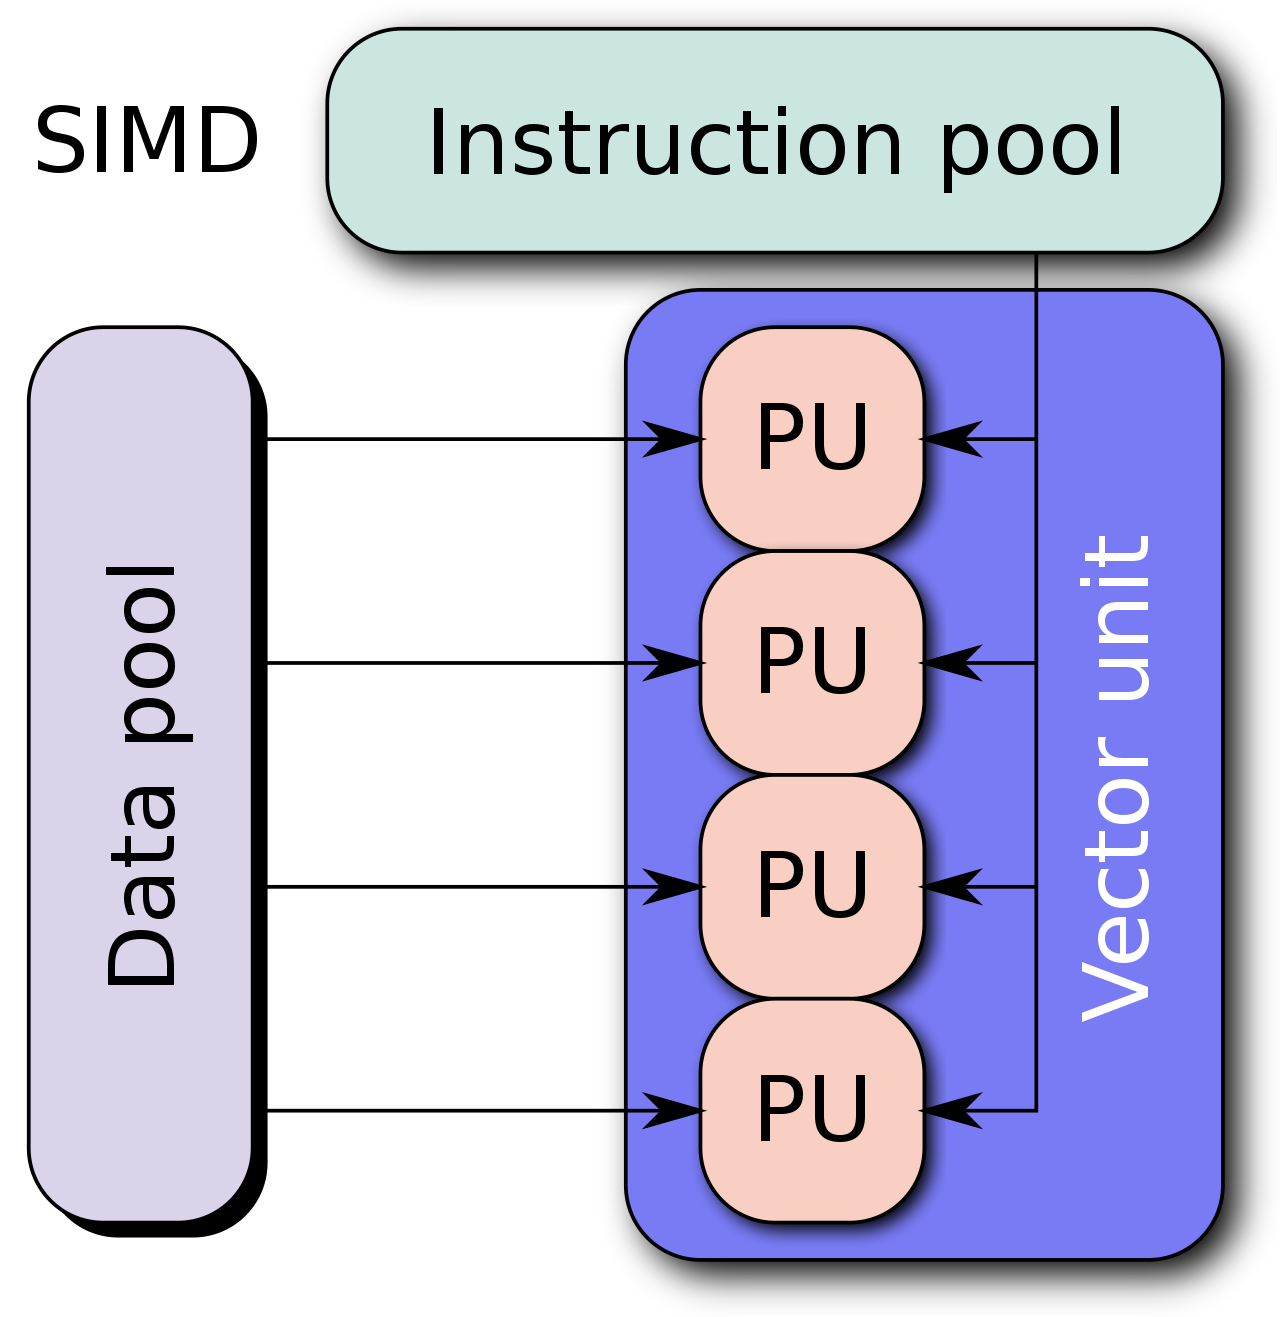
\includegraphics[height=0.5\textheight]{images/SIMD2.svg.png}
        \caption{SIMD}
    \end{figure}

\end{frame}

\begin{frame}
    \frametitle{Benefits of SIMD}

    通常情况下我们很难将串行代码转化为并行,为了设计并行算法通常需要改变原有的
    逻辑。

    \begin{figure}[h]
        \centering
        
\includegraphics[width=0.5\textwidth]{images/rgba.png}
        \caption{RGBA}
    \end{figure}

    如图所示,在图形学中我们经常需要计算图像的颜色信息,而颜色在RGBA几个维度下
    的计算是可以向量化的。

\end{frame}


\begin{frame}
    \frametitle{GPGPU}

    显卡(GPU)包含大量的核心来支持高度并行化的计算,最开始的在显卡上的编程是很困
    难的,随着时代的发展显卡的计算能力越来越不容小觑,通用计算显卡(GPGPU)也开始
    包含在编译优化的领域。如何把科研大佬写的模型,放到真正的显卡上执行?

    \begin{figure}[h]
        \centering
        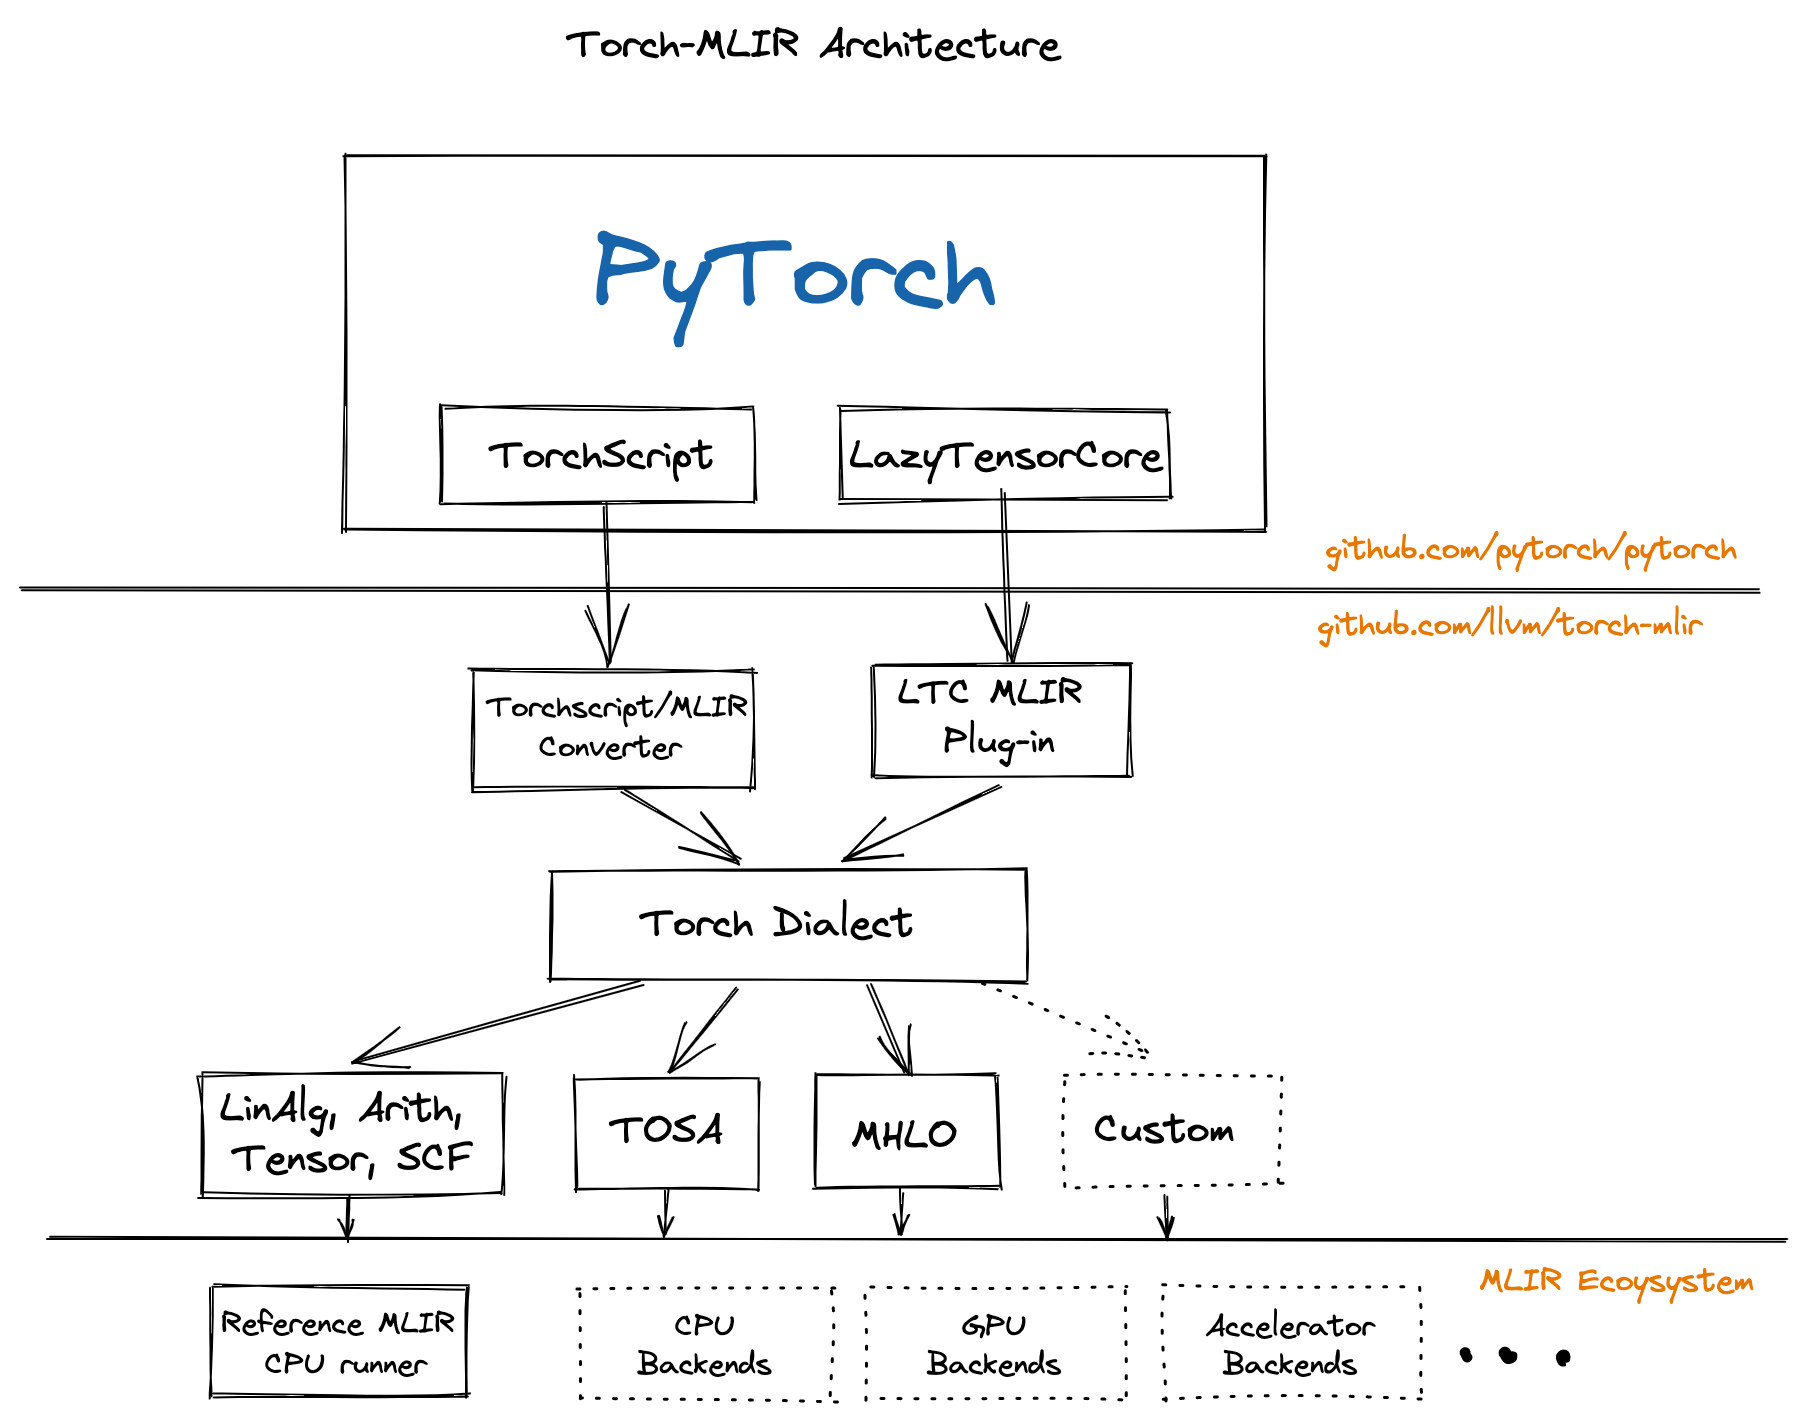
\includegraphics[height=0.5\textheight]{images/torch-mlir.png}
        \caption{Torch-MLIR}
    \end{figure}

\end{frame}

\begin{frame}
    \frametitle{Problem With SIMD Instructions}

    \begin{block}{RISC-V Designers}
        \textit{SIMD Instructions considered harmful. -- David Patterson}
    \end{block}

    一开始,SIMD被认为是实现并行化简单有效的方法。我们将64位寄存器和ALU划分为许
    多8, 16, 32位的块,然后并行地计算它们。用每条指令的操作码(opcode)提供数据宽
    度和操作。

    \textbf{指令集膨胀}

    IA-32指令集已经从最开始的80多条指令增长到了现在的1400多条。SSE, AVX, 各种
    SIMD扩展和宽寄存器让指令集变得越来越复杂。
\end{frame}

\begin{frame}[fragile]
    \frametitle{Vector vs SIMD}

    向量机与SIMD的真正区别在于,向量长度是否在机器码层面确定。

    \begin{lstlisting}
void *memcpy_vec(void *dst, void *src, size_t n) {
    void *save = dst;
    // copy data byte by byte
    for (size_t vl; n > 0; n -= vl, src += vl, dst += vl) {
        vl = vsetvl_e8m8(n);
        vuint8m8_t vec_src = vle8_v_u8m8(src, vl);
        vse8_v_u8m8(dst, vec_src, vl);
    }
    return save;
}
    \end{lstlisting}


\end{frame}

\section{Auto-Vectorization}

\begin{frame}[fragile]
    \frametitle{Auto-Vectorization}

    标量代码可以被自动向量化成含向量计算的代码。

    事实上,大量的标量循环都可以被向量化

    \begin{lstlisting}
void add(int * restrict A, int * restrict B, int n){
    for(int i = 0;i < n;i++){
        A[i] += B[i];
    }
}
    \end{lstlisting}


\end{frame}

\begin{frame}[fragile]
    \frametitle{合法性}

    数据依赖 \& Overlap (Alias Analysis)

    \begin{lstlisting}
for (int i = 0; i < N; i += 1) {
    a[i+1] = b[i] + 1;  // S1
    b[i+1] = a[i] + 1;  // S2
}
    \end{lstlisting}

    \begin{figure}
        \centering
        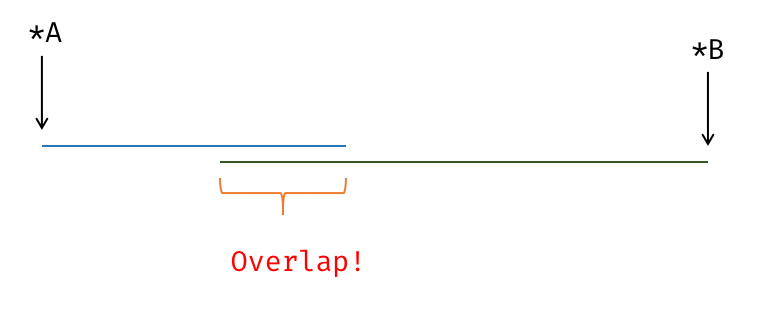
\includegraphics[width=0.4\textwidth]{images/overlap.png}
        \caption{Example of pointer overlapping}
    \end{figure}

\end{frame}

\begin{frame}[fragile]
    \frametitle{合法性}

    \begin{lstlisting}
for(int i = 1;i < n;i++)
    A[i] = A[i - 1];
    \end{lstlisting}
    \begin{lstlisting}
for(int i = 1;i < n;i++)
    A[i + 1] = B[i]; // overlap?
    \end{lstlisting}

    \begin{figure}
        \centering
        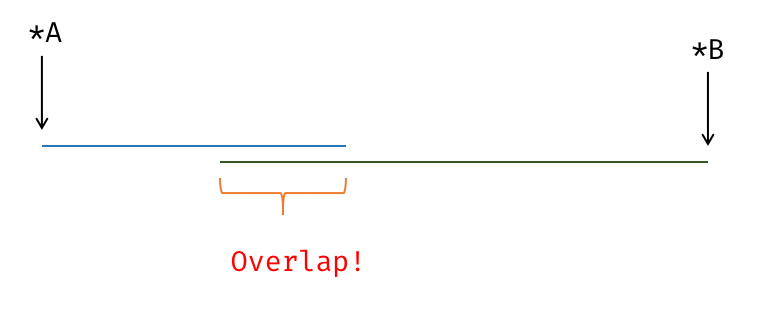
\includegraphics[width=0.4\textwidth]{images/overlap.png}
        \caption{Example of pointer overlapping}
    \end{figure}

\end{frame}

\begin{frame}[fragile]
    \frametitle{收益}

    必然导致的程序大小增加 / 标量循环和向量循环的选择和跳转

    数据对齐的代价,尾循环的代价,都是需要考虑的因素。

    \begin{minipage}[t]{0.45\linewidth}
        \begin{lstlisting}[language=C++]
load i64;
load i64;
load i64;
load i64;
        \end{lstlisting}
    \end{minipage}
    \begin{minipage}[t]{0.45\linewidth}
        \begin{lstlisting}[language={[RISC-V]Assembler}]
load <4 x i64>;
        \end{lstlisting}
    \end{minipage}

    由体系结构实现。

\end{frame}

\begin{frame}
    \frametitle{Transformation}

    \begin{figure}
        \centering
        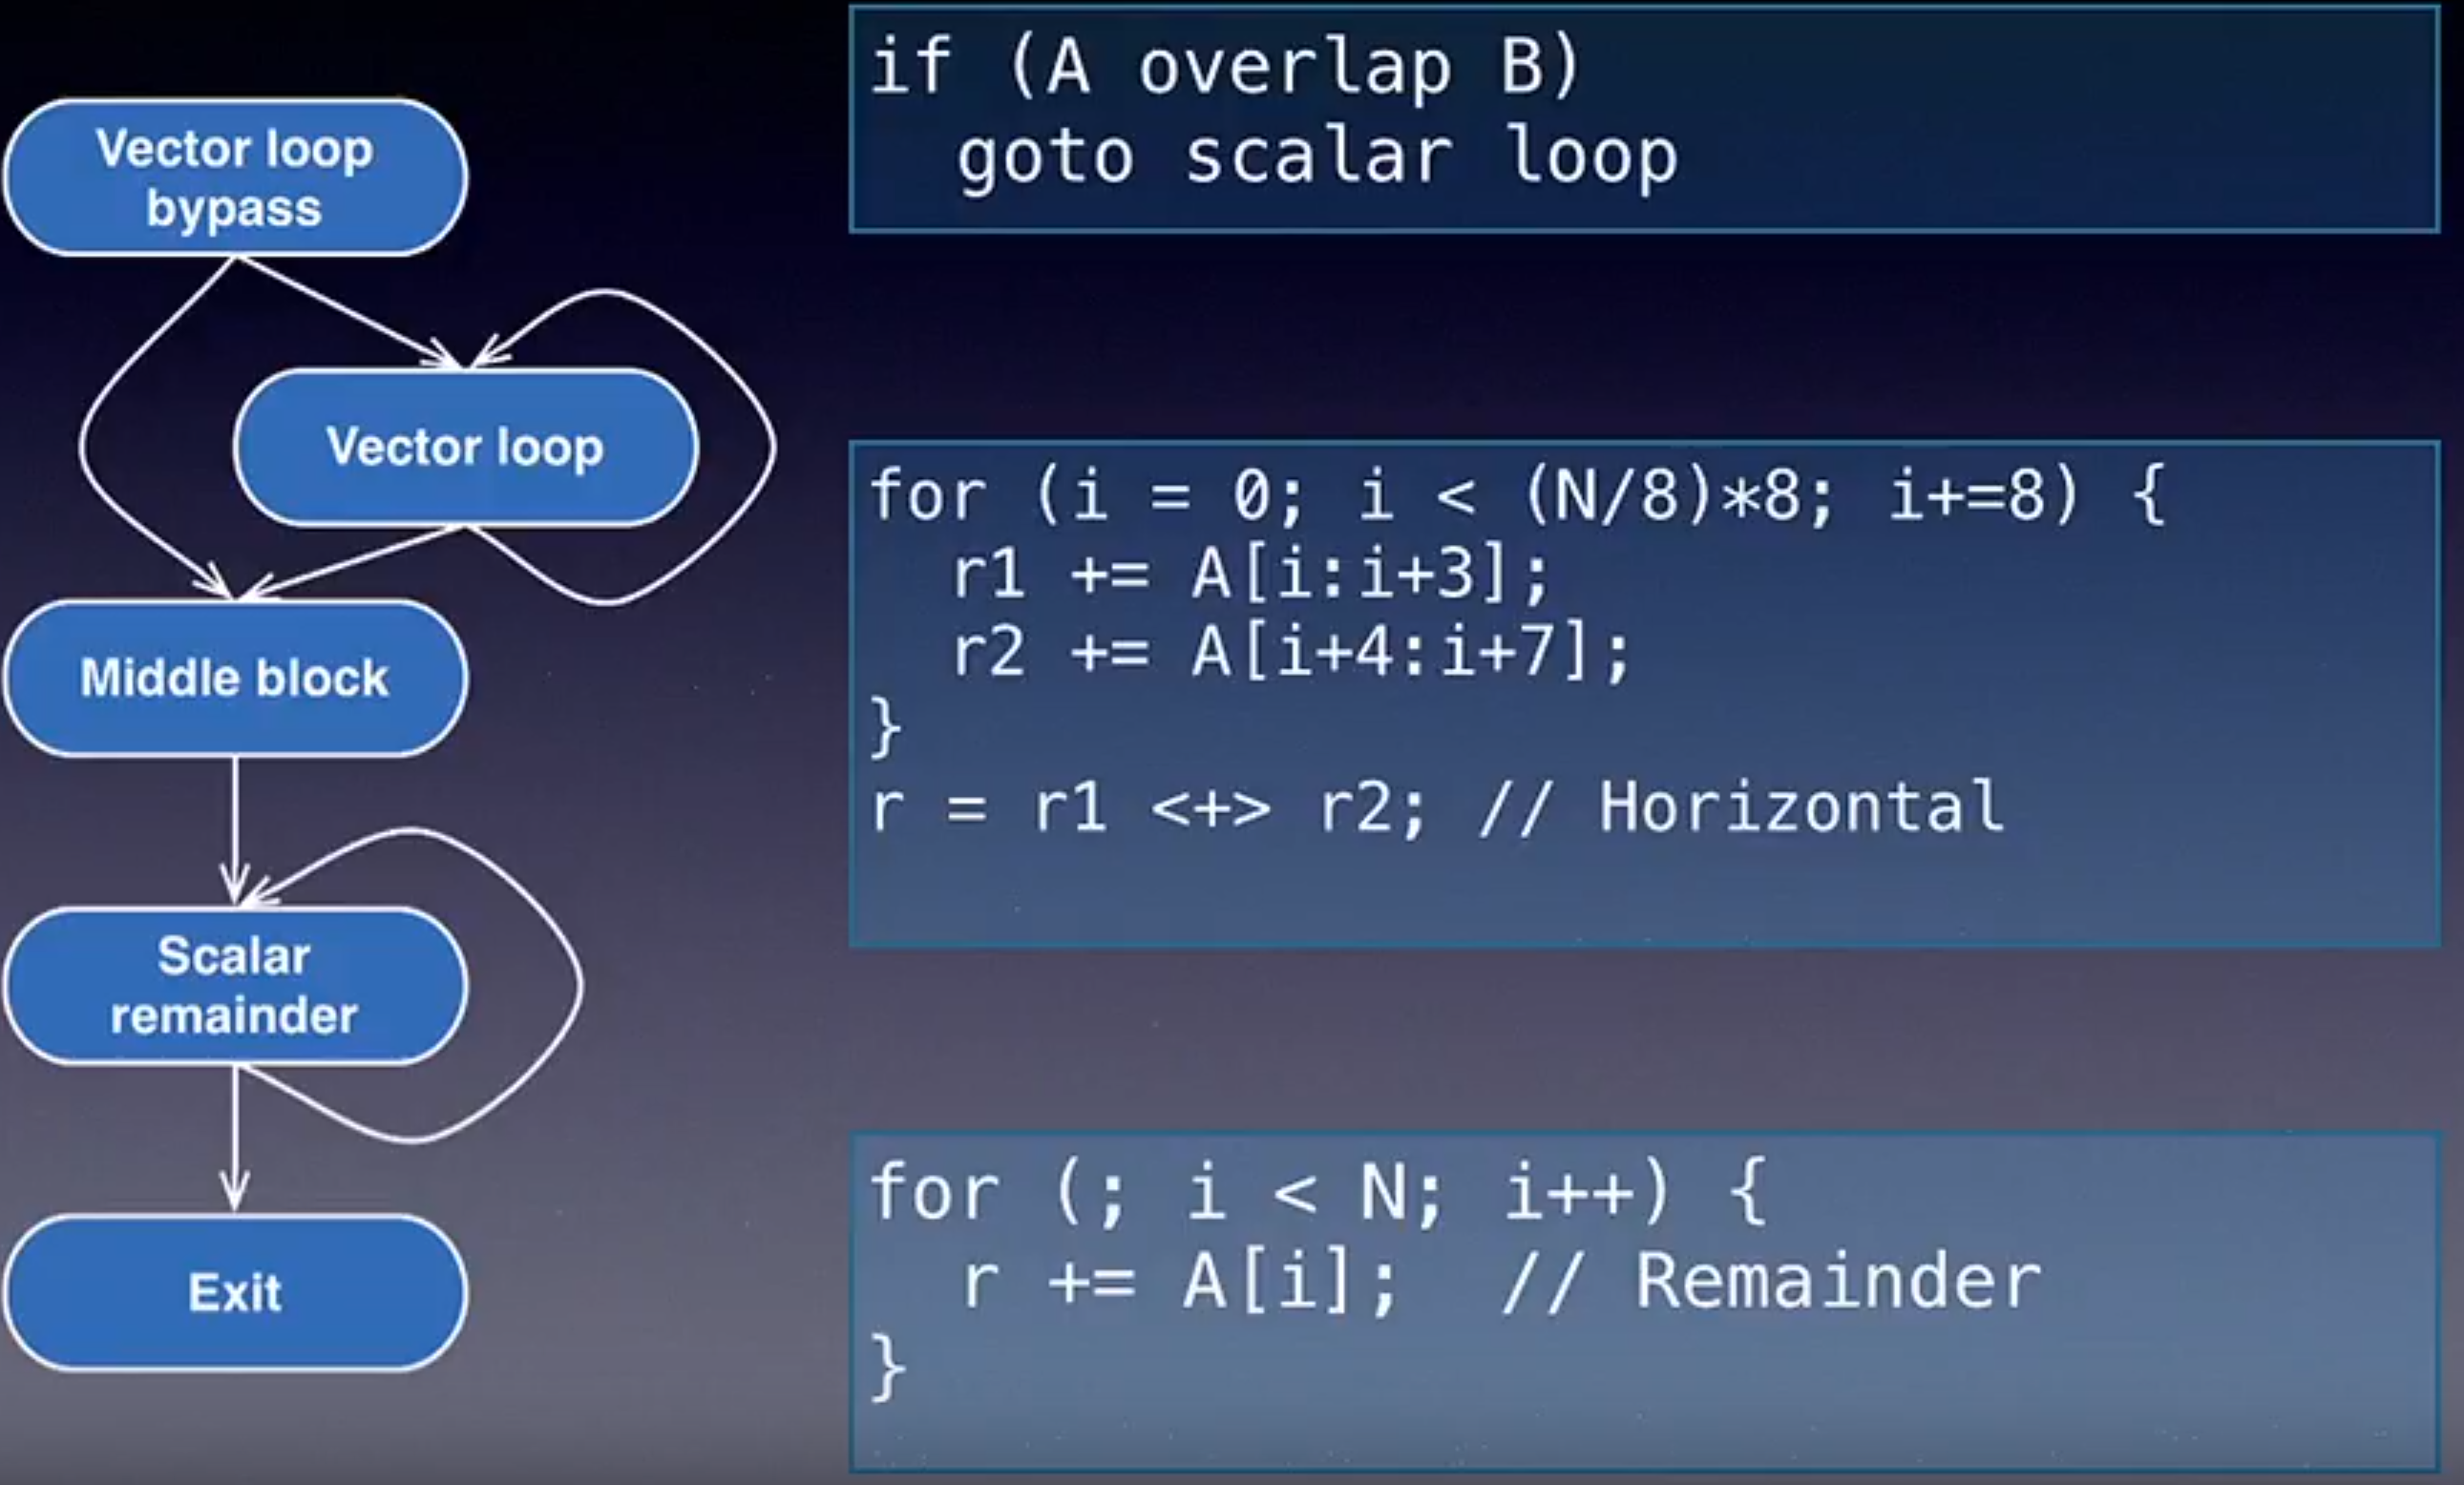
\includegraphics[width=0.6\textwidth]{images/trans.png}
        \caption{LLVM Developer 2013 by Apple}
    \end{figure}

\end{frame}

\begin{frame}[fragile]
    \frametitle{Loop Vectorizer Enhancements}

    现代化向量指令集可以更好地完成向量长度选择。

    \begin{lstlisting}[language={[RISC-V]Assembler}]
memcpy:
    mv a3, a0 # Copy destination
loop:
    vsetvli t0, a2, e8, m8, ta, ma   # Vectors of 8b
    vle8.v v0, (a1)                  # Load bytes
    add a1, a1, t0                   # Bump pointer
    sub a2, a2, t0                   # Decrement count
    vse8.v v0, (a3)                  # Store bytes
    add a3, a3, t0                   # Bump pointer
    bnez a2, loop                    # Any more?
    ret                              # Return
    \end{lstlisting}

\end{frame}

\begin{frame}
    \frametitle{Mask \& Predication}

    Predication (判定寄存器) 其实是来源于ARM SVE的一个东西

    VP-based Loop Vectorizer 在 LLVM 中还没实现...

\end{frame}

\subsection{Challenges}
\begin{frame}
    \frametitle{Challenges - 并行的多样性}

    并行是目前主要算力,但是 ISA 定义多样。我们难以找到一个合适的抽象来用统一的范式进行自动向量化。

    \begin{table}
        \centering
        \caption{不同运算设备并行设计与实现}
        \scriptsize
        \begin{tabular}{ccc}
            \toprule
            设备 / ISA         & 对应的并行实现                             & 备注           \\
            \midrule
            NVIDIA/AMD GPU   & SIMT                                & 结合 SIMD 和多线程 \\
            寒武纪              & SIMD 长度可变                           & repeat 操作    \\
            升腾               & 默认操作 tensor                         & 看起来可能是多维的    \\
            以 x86 为代表的传统 CPU & 定长,通常可以同时操作标量                       & 需要对齐、尾循环处理等  \\
            RISC-V           & scatter \& gather, \& 长度可变, \& mask & V 扩展         \\
            ARM-SVE          & 类似 RVV                              & 没有 RVV 灵活    \\
            \bottomrule
        \end{tabular}
    \end{table}

    编译器难以使用统一的范式进行自动向量化。

\end{frame}

\subsection{Prior Art}

\begin{frame}
    \frametitle{Prior Art - MLIR \& LLVM}

    \begin{enumerate}
        \item MLIR - 目前没有自动向量化 \\
              Vector Dialect,面向各种 DSL 提供 n-D vector type,并可以在 lowering 到 LLVM IR 的过程中对 n-D vector 进行 re-layout,例如组成float4,
        \item LLVM - 有向量化,但主要面向传统 CPU \\
              从引入 Vector Predication 开始,主要被作为 CodeGen 的最后一关对接 MLIR,LLVM 本身的自动向量化有较大历史包袱。
    \end{enumerate}
\end{frame}

\subsection{Goal}

\begin{frame}
    \frametitle{Goal - Auto-Vectorization Service}

    \begin{enumerate}
        \item Extensible: 足够方便扩展
        \item Composible: 可以组合各种情况
        \item Simple: IR 层面尽量显然,避免多余静态分析
    \end{enumerate}
\end{frame}

\section{Virtual Vector - \texttt{vector} Dialect}

\begin{frame}
    \frametitle{Virtual Vector}

    MLIR \texttt{vector} Dialect 提供了对各种向量的平台无关的丰富抽象.

    作为核心数据类型的 vector 可以是:
    \begin{itemize}
        \item 多维的, 或不确定维数的
        \item 定长的, 或不确定长度的, 或变长的
        \item 可以包含几乎任意的基本数据类型, 甚至诸如 int4 等类型
    \end{itemize}

    能表示 vector 在各种层次上的操作:
    \begin{itemize}
        \item 基本的创建, 运算, 内存读写, 元素读写
        \item 贴合 LLVM intrinsic 级别的操作 (e.g. 各种底层 load/store, 一维向量操作)
        \item 一般向量操作 (e.g. reduce)
        \item 贴合 Linalg 级别的操作 (e.g. transfer\_read, transfer\_write, contract)
    \end{itemize}
\end{frame}

\begin{frame}[fragile]
    \frametitle{HPC \& nD vector}
    MLIR Vector Dialect 提供了一个 nD vector 的抽象。这种抽象对于现代 HPC 来说是必要的。
    一个简单的例子:

    \begin{lstlisting}
kernel (float4 A).     load A[0-3]; add[0-3]
kernel (float A).     load A[0-15]; add[0-3]; add[4-7]; add[8-11]; add[12-15]

vector A[25 x float4] => A[25 x 4 x float]
    \end{lstlisting}
\end{frame}



\begin{frame}
    \frametitle{Position}
    \begin{minipage}[t]{0.47\textwidth}
        \small
        \begin{itemize}
            \item \texttt{affine/scf} 等上层 Dialect 解决循环等结构操作
            \item \texttt{arith} 等基本 Dialect 完成基本的向量创建和四则运算
            \item 各种 ISA-spec Dialect 补充自己没有的底层细节
            \item \texttt{vector} 则集中表示 ``通用'' 的向量操作
        \end{itemize}
    \end{minipage}%
    % \hfill%
    \begin{minipage}[t]{0.5\textwidth}
        \begin{figure}
            \centering
            \includegraphics[width=1.0\linewidth]{images/position.png}
            \caption{Positioning in the Codegen Infrastructure}
        \end{figure}
    \end{minipage}
\end{frame}

\begin{frame}
    \frametitle{Virtual Vector Lowering Path}
    \noindent
    \begin{minipage}[t]{0.50\linewidth}
        \begin{figure}
            \centering
            \includegraphics[width=1.0\linewidth]{images/position2.png}
            \caption{MLIR Patterns}
        \end{figure}
    \end{minipage}%
    \hfill%
    \begin{minipage}[t]{0.45\linewidth}
        主要的三层中间表达:
        \begin{enumerate}
            \item Virtual Vector:使用nD vector type,\texttt{vector<4x8x128xf32>}
            \item Hardware Vector:Op $\approx$ 指令
            \item LLVM:instructions,intrinsics, $\dots$
        \end{enumerate}

        \begin{itemize}
            \item VV同层转换:例如unroll,permute
            \item VV $\rightarrow$ HWV,一些手写的pattern:例如CPU的VL;这层lower之后,一些循环优化被禁止(需要确认)
            \item HWV $\rightarrow$ LLVM,手工的
        \end{itemize}
    \end{minipage}
\end{frame}

\begin{frame}
    \frametitle{Language Lowering Path}
    \begin{figure}
        \centering
        \includegraphics[width=0.35\linewidth]{images/auto-vec-path.png}
        \caption{Lowering path from language to ISA}
    \end{figure}
\end{frame}

\begin{frame}
    \frametitle{Auto-Vectorization $\Rightarrow$ Pattern-Rewrite?}

    总体思路:自动向量化 $\rightarrow$ 将标量提升为 Vector 类型 $\rightarrow$ Aseembly

    \hspace{2em}

    如果源代码:
    \begin{enumerate}
        \item 矩阵乘法等高维形式: DSL $\rightarrow$ \texttt{linalg} ($\rightarrow$ \texttt{affine} $\rightarrow$) $\rightarrow$ \texttt{vector}
        \item 标量循环: \texttt{scf.for}/通用语言 $\rightarrow$ \texttt{affine.for} $\rightarrow$ \texttt{vector}
    \end{enumerate}

    \begin{center}
        \vspace{2em}
        挑战:如何将标量循环转换为 \texttt{vector} ?
    \end{center}

\end{frame}

\begin{frame}
    \frametitle{标量循环 $\rightarrow$ \texttt{vector} Dialect}

    \begin{center}
        挑战:如何将标量循环转换为 \texttt{vector} ?

        \vspace{1.5em}
    \end{center}

    \begin{enumerate}
        \item 从标量循环/scf/语言分析数据访问和依赖
        \item 尽可能识别特定模式并生成 \texttt{affine.for}
        \item 在 \texttt{affine} 上做嵌套循环相关的优化(例如 loop fusion, unroll 等)
        \item 再在 \texttt{affine} 上做向量化 (例如 \texttt{SuperVectorize.cpp})
    \end{enumerate}
\end{frame}

\begin{frame}[fragile]
    \frametitle{C for-loop $\rightarrow$ basic \texttt{affine} Dialect}
    \noindent
    \begin{minipage}[t]{0.3\linewidth}
        \lstinputlisting[language=C,basicstyle=\Tiny]{assets/example.c}
        \begin{itemize}
            \scriptsize
            \item 源代码 $\rightarrow$ \texttt{affine} ?
            \item scf.for $\rightarrow$ \texttt{affine.for} 简单
            \item scf.while $\rightarrow$ \texttt{affine.for} 复杂
        \end{itemize}
    \end{minipage}%
    \hfill%
    \begin{minipage}[t]{0.6\linewidth}
        \lstinputlisting[language=llvm,basicstyle=\Tiny]{assets/example_direct_affine.mlir}
    \end{minipage}
\end{frame}

\begin{frame}[fragile]
    \frametitle{Loop Normalization on \texttt{affine} Dialect}

    \begin{minipage}[t]{0.6\linewidth}
        \lstinputlisting[language=llvm]{assets/example_normalized.mlir}
    \end{minipage}%
    \hfill%
    \begin{minipage}[t]{0.4\linewidth}
        \vspace{3em}
        除了循环正规化, 在 \texttt{scf} 和 \texttt{affine} dialect 上有一些现存的循环变换 pass, 可以通过 \texttt{mlir-opt --help} 查看.
    \end{minipage}

\end{frame}

\begin{frame}[fragile]
    \frametitle{Induction Variable Elimination on \texttt{affine} Dialect}

    \lstinputlisting[language=llvm]{assets/indvars.mlir}
\end{frame}

\begin{frame}[fragile]
    \frametitle{Final Result}

    \lstinputlisting[language=llvm]{assets/final.mlir}
\end{frame}

\begin{frame}[fragile]
    \frametitle{\texttt{affine} $\rightarrow$ \texttt{vector}}

    \begin{lstlisting}[language=llvm]
// send it to affine-supre-vertorize pass
// mlir-opt --affine-super-vectorize='virtual-vector-size=256 test-fastest-varying=0'
func.func @example_vector() {
    //... same as above
    // unimplement yet :(
    func.return
}
    \end{lstlisting}

    目前的 \texttt{affine} super-vectorize 只实现了少量 case !

\end{frame}

\begin{frame}[fragile]
    \frametitle{\texttt{affine} $\rightarrow$ \texttt{vector}}

    一个真实可用的例子:

    \lstinputlisting[language=llvm]{assets/affine-a+b.mlir}

    上面的 $C = A + B$ 可以被变为:

    \lstinputlisting[language=llvm]{assets/affine-vec.mlir}

\end{frame}

\begin{frame}
    \frametitle{Target Feature}

    一些体系结构支持 \texttt{vector} Dialect 之外的其他扩展,如何充分利用体系结构的能力?

    \vspace{1.5em}

    \begin{enumerate}
        \item 定义自己的 Dialect ,作为 \texttt{vector} Dialect 的补充
        \item Custom Vectorizer
        \item Lowering Path
    \end{enumerate}

\end{frame}


\begin{frame}
    \frametitle{Conclusion}

    对于某一个新体系结构,要想针对其实现自动向量化,可以的方案:

    \begin{enumerate}
        \item 观察 \texttt{vector} Dialect 有没有已有的抽象,将没有的抽象自定义 Dialect
        \item 自己实现自定义 Dialect 的自动向量化
        \item 自定义 Dialect 离开 MLIR 后,需要有基础设施 Lowering 到 asm (LLVM, NVVM,SPIR-V)
    \end{enumerate}

\end{frame}

\section{RISC-V V Extension}

\begin{frame}
    \frametitle{RISC-V}

    RVV 被认为是面向``超级计算机''的扩展。RVV 支持多种现代向量指令集所具有的操作,从编译器设计角度带来了一些具体的挑战:

    \begin{table}
        \scriptsize
        \centering
        \caption{部分 RVV Feature 与对应编译器自动向量化实现情况}
        \begin{tabular}{cccc}
            \toprule
            RVV Feature         & 功能           & 传统 SIMD       & LLVM 实现             \\
            \midrule
            向量长度寄存器 \texttt{vl} & 控制要执行的向量长    & 无             & VP,向量化忽略            \\
            mask                & mask 掉不需要的   & 有,较少 (AVX512) & VP,向量化忽略            \\
            寄存器编组               & 向量寄存器可以组合或拆分 & 以不同指令区分不同向量长度 & \thead{基于 vscale 实现 \\ 向量化需要手动指定} \\
            \bottomrule
        \end{tabular}
    \end{table}

\end{frame}

\begin{frame}{Current RVV Vectorization Lowering Path}
    \begin{minipage}[t]{0.5\textwidth}
        \begin{table}
            \scriptsize
            \centering
            \caption{MLIR Lowering Path 实现情况}
            \begin{tabular}{ccc}
                \toprule
                序号                                                                                                                            & 实现情况 & 备注           \\
                \midrule
                (1)                                                                                                                           & 无    & 有参考资料        \\
                (2)\footnote{\tiny 可以在循环主体部分参考 SIMD 架构的实现, 循环尾的处理需要新的实现}                                                                      & 无    & 无(少)参考资料     \\
                (3) (6)                                                                                                                       & 成熟   &              \\
                (4)(5)\footnote{\tiny 基本无实现,需要对现有代码较大增补和验证,并且需要和上游交流,例如 Scalable 与非 Scalable 的混杂、原来的对 operation 的递归定义是否对 Scalable Vector 适用?} & 无    & Scalable 新加入 \\
                \bottomrule
            \end{tabular}
        \end{table}

        \scriptsize
        LLVM 后端有 vector intrinsic 和 vp intrinsic 两种后端可选。

        其中 vp 出现较晚,没有 vector 成熟,但基本能用。
    \end{minipage}%
    % \hfill%
    \begin{minipage}[t]{0.5\textwidth}
        \begin{figure}
            \centering
            \includegraphics[width=0.5\linewidth]{images/lowering-path-around-vector.png}
            \caption{Lowering path around vector dialect}
        \end{figure}
    \end{minipage}
\end{frame}

\end{document}
